\documentclass[12pt]{article}
\usepackage[margin=1in]{geometry}
\usepackage{float}
\usepackage{multicol}
\usepackage{lmodern}
\usepackage{amssymb,amsmath}
\usepackage{ifxetex,ifluatex}
\usepackage{fixltx2e} % provides \textsubscript
\ifnum 0\ifxetex 1\fi\ifluatex 1\fi=0 % if pdftex
  \usepackage[T1]{fontenc}
  \usepackage[utf8]{inputenc}
\else % if luatex or xelatex
  \ifxetex
    \usepackage{mathspec}
    \usepackage{xltxtra,xunicode}
  \else
    \usepackage{fontspec}
  \fi
  \defaultfontfeatures{Mapping=tex-text,Scale=MatchLowercase}
  \newcommand{\euro}{€}
\fi
% use upquote if available, for straight quotes in verbatim environments
\IfFileExists{upquote.sty}{\usepackage{upquote}}{}
% use microtype if available
\IfFileExists{microtype.sty}{%
\usepackage{microtype}
\UseMicrotypeSet[protrusion]{basicmath} % disable protrusion for tt fonts
}{}
\usepackage{graphicx}
\makeatletter
\def\maxwidth{\ifdim\Gin@nat@width>\linewidth\linewidth\else\Gin@nat@width\fi}
\def\maxheight{\ifdim\Gin@nat@height>\textheight\textheight\else\Gin@nat@height\fi}
\makeatother
% Scale images if necessary, so that they will not overflow the page
% margins by default, and it is still possible to overwrite the defaults
% using explicit options in \includegraphics[width, height, ...]{}
\setkeys{Gin}{width=\maxwidth,height=\maxheight,keepaspectratio}
\ifxetex
  \usepackage[setpagesize=false, % page size defined by xetex
              unicode=false, % unicode breaks when used with xetex
              xetex]{hyperref}
\else
  \usepackage[unicode=true]{hyperref}
\fi
\hypersetup{breaklinks=true,
            bookmarks=true,
            pdfauthor={Brandon LeBeau},
            pdftitle={PSQF 4143: Section 2 Supplemental},
            colorlinks=true,
            citecolor=blue,
            urlcolor=blue,
            linkcolor=magenta,
            pdfborder={0 0 0}}
\urlstyle{same}  % don't use monospace font for urls
\setlength{\parindent}{0pt}
\setlength{\parskip}{6pt plus 2pt minus 1pt}
\setlength{\emergencystretch}{3em}  % prevent overfull lines
\setcounter{secnumdepth}{0}

\title{PSQF 4143: Section 2 Supplemental}
\author{Brandon LeBeau}
\date{}

\begin{document}
\maketitle

\section{Frequency Polygons}\label{frequency-polygons}

\begin{itemize}
\itemsep1pt\parskip0pt\parsep0pt
\item
  Similar to a histogram, but the frequency are plotted above the
  midpoint of each interval.
\item
  The midpoint is the middle of the interval taking into account the
  real limits.

  \begin{itemize}
  \itemsep1pt\parskip0pt\parsep0pt
  \item
    \(mid = X_{ll} + \frac{(X_{ul} - X_{ll})}{2}\)
  \end{itemize}
\end{itemize}

\begin{verbatim}
##         Var1 Freq midpoint
## 1    [80,90)    1     84.5
## 2   [90,100)    6     94.5
## 3  [100,110)    6    104.5
## 4  [110,120)    2    114.5
## 5  [120,130)    6    124.5
## 6  [130,140)    4    134.5
## 7  [140,150)    3    144.5
## 8  [150,160)    0    154.5
## 9  [160,170)    1    164.5
## 10 [170,180)    1    174.5
\end{verbatim}

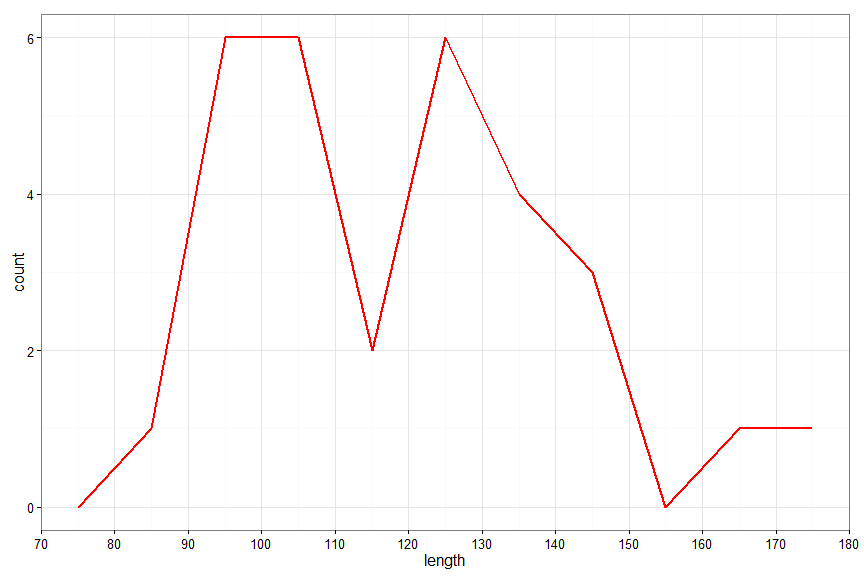
\includegraphics[width=3.5in]{figure/freqpoly-1.png}
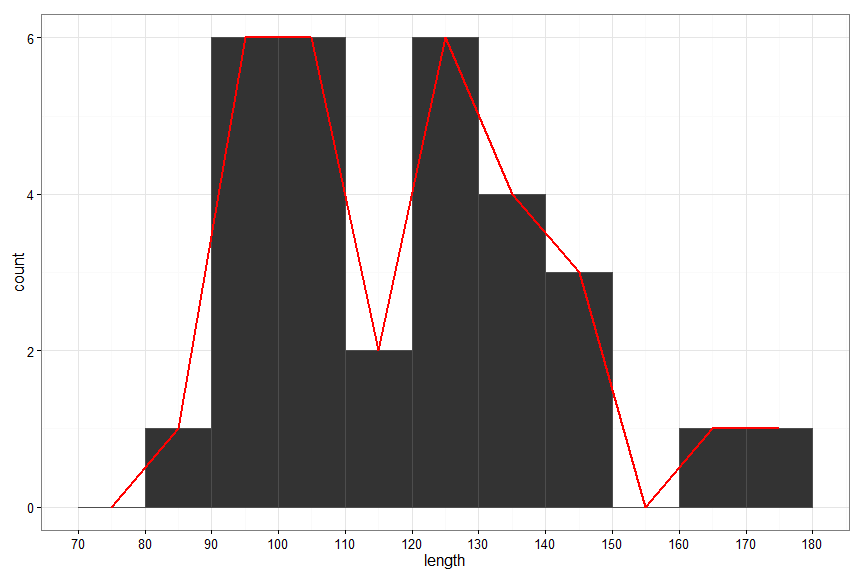
\includegraphics[width=3.5in]{figure/freqpoly-2.png} \\
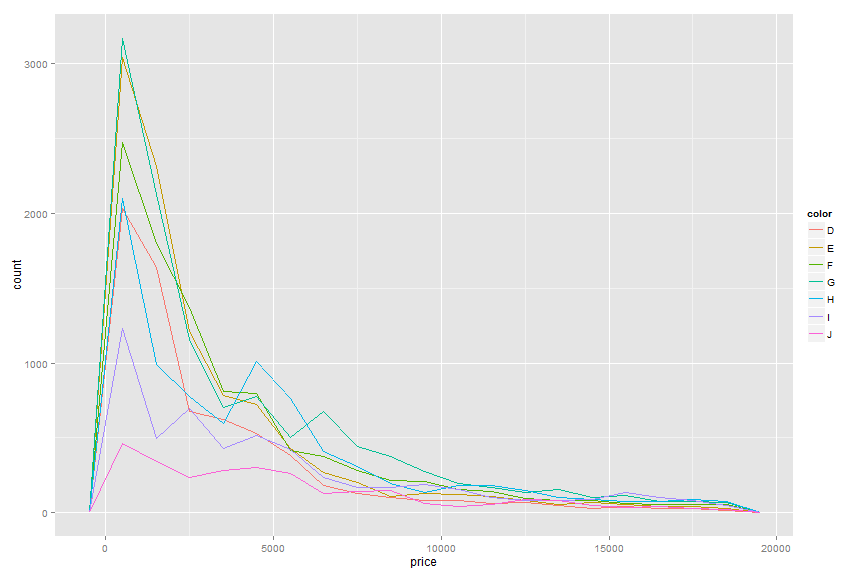
\includegraphics[width=3.5in]{figure/freqpoly-3.png}

\section{Stem and Leaf}\label{stem-and-leaf}

\begin{itemize}
\itemsep1pt\parskip0pt\parsep0pt
\item
  The leaf is the last digit of the number
\item
  The stem is everything except for the last digit.
\end{itemize}

\begin{verbatim}
## 
##   The decimal point is 1 digit(s) to the right of the |
## 
##    8 | 6
##    9 | 257899
##   10 | 048899
##   11 | 03
##   12 | 001347
##   13 | 2226
##   14 | 013
##   15 | 
##   16 | 2
##   17 | 0
\end{verbatim}

\end{document}
